\section{Problem 2}

In this problem we analyse the Vandermonde matrix and use various techniques to solve it. The way I formatted this is by first listing the whole code, and then per sub-question discussing the output of relevant part of the code. I did this because some of the code overlaps between sub-questions. Per sub-question, I indicate in the code the part relevant to it (e.g. \#2A). The very beginning is copied from the recommended routine of the Exercise set, as well as some plots. The code I have written is as follows: 

\lstinputlisting{NURhandin1_2.py}

\subsection{Problem 2a}

First we take a look at problem 2a. In this problem, the goal is to write a code that does an LU decomposition of the Vandermonde matrix and use the resulting LU matrix to obtain the solutions $c_i$ for data points $x_i$, where i = 0,1,...,19. First of all, we create the matrix V. We do this by taking every row to be (1, $x_i$, $x_{i}^2$, ...., $x_{i}^{19}$), again for our different 20 data values $x_i$, filling j = 1,2,...,19 rows in total. In order to first obtain the LU matrix, we apply the $\textbf{improved Crout's algorithm}$ from lecture 3 slide 15 as shown in the code. As can be seen in the code, we first take our LU matrix as the input matrix V (as instructed on slide 13), and gradually swap and overwrite different elements of the matrix. If an input matrix is not square, we return an error message that no LU matrix can be found for a singular matrix. All used for loops can be translated to summing for different values i within the range of the loop. The if-statements determine the conditions for which we should apply operations. After we finish all loops, we return a matrix LU of equivalent shape to V that contains our $\alpha_{ij}$ and $\beta_{ij}$ values, which we will require to apply forward- and backward substitution.\\

Next, using the LU matrix and the given b=$y_i$ data values, we apply a $\textbf{forward subtitution algorithm}$ inspired by slide 11 of lecture 3. The diving by $\alpha_{ii}$ factors are omitted because we have set these values to be equal to 1 implicitly. From this rather straightforward algorithm, we (confusingly) obtain the y values we require to apply $\textbf{backward subtitution}$. This algorithm is a bit more complicated. We go through this loop in reverse order, applying numerous operations to construct our solution vector x. These operations include dividing by $\beta_{ii}$ and multiplying by $\beta_{ij}$ and $y_i$ values respectively for j $>$ i, opposite from the conditions from the forward subtitution, j $<$ i. Finally, we combine these three seperate algorithms into a final function in which we can input the matrix we want to solve A and it's solution b. In our case, we will use V and y respectively for this. This function then returns a vector of x-values. These are the c-values we wished to obtain, given by:

\lstinputlisting{problem2a.txt}

Using these c values, we can calculate (interpolate) the y values by applying equation (2) from the hand-in set with the 1000 x values we want to interpolate at. Next, we plot the resulting 1000 y values together with the 20 y points from the data to see how they match:

\begin{figure}[h!]
  \centering
  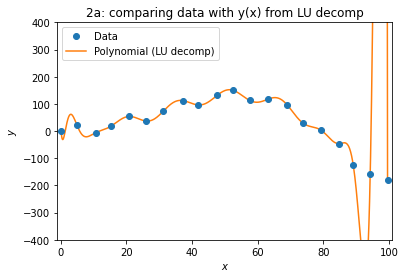
\includegraphics[width=0.6\linewidth]{problem2a1.png}
  \caption{The polynomial y(x) obtained with the LU decomposition method plotted together with the given data points to test whether it intersects them.}
  \label{fig:fig1}
\end{figure}

From this figure we can conclude that we get a pretty good description of the data, except for x values below 5 and especially above 90. At x values close to the maximum, the polymial seems to vary wildy. Despite this, it still does go through the data points somewhat well as seen in the plot. The accuracy does decrease at these higher x values though, as can be seen in the second plot below, where we calculate the absolute value of the error per data point:

\begin{figure}[h!]
  \centering
  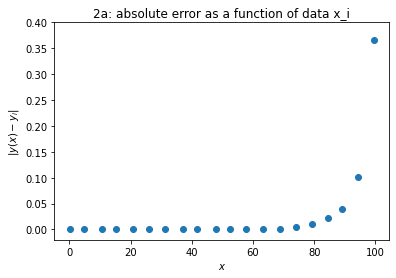
\includegraphics[width=0.6\linewidth]{problem2a2.png}
  \caption{The absolute difference between the polynomial y(x) and the data points $y_i$ to visualise how far off the polynomial is from the actual data. This y-scale seemed most appropiate as it still includes the point with the highest error value. Smaller y limit values barely show any error in the lower x values regardless.}
  \label{fig:fig2}
\end{figure}

All in all, the result is quite satisfactory, as both visually and quantitatively, the polynomial seems to describe the data points fairly well, save for the aforementioned boundary cases. 

\subsection{Problem 2b}

For this next sub-question, we are supposed to implement $\textbf{Neville's algorithm}$ to find interpolated y values for a given input array of x values between 0 and 20. To apply this algorithm, we first write a $\textbf{bisection algorithm}$ to find the index $j_{low}$, which is the closest index to the index of our x value we want to interpolate at. In our bisection algorithm, we first treat the cases were there is extrapolation, meaning the x value falls outside of the range of xdata values. In this case, we simply take the indices around the edges to interpolate with like in problem 1 of tutorial 2. Next, we set up a start, end and size index. An important note is the way the algorithm is written, the start index will be equivalent to the $j_{low}$ index and will be updated as we continue. From these we can implicitly construct a left and right half range of indices of the sample values. After this, we go into a while loop and update our left and right index ranges as we continue to narrow down the ranges. We quit this process once we find that the difference in start and end indices falls below 1, because that means the indices start to overlap, which is something we want to avoid as at this point we already found the closest indices. After we reach this threshold, we take the start value, which is the lower closest index (the value is floored), and compare this for a set of cases. If this index (remember this is $j_{low}$) is either smaller than the given order or the index plus the order exceed the amount of data points, we return 0 and $j_{low} - order$ respectively. For the non-edge cases however, we obtain the smallest index $j_{low}$.\\

From $j_{low}$ we find the total range of M tabulated points around x given by $[j_{low},j_{low}+M]$. As we have a 19th degree polynomial in this case, we use an input value of M = 20, as this is equivalent to order (M-1 =) 19. 